\documentclass[aspectratio=169]{beamer}
\usepackage[english]{babel}
\usepackage{dsfont}
\usepackage{tabularx}
\input{preamble}
\title{Evaluation of gate designs} %->->->->-> Check hyperref title <-<-<-<-<-
\subtitle{For trapped ion quantum computers}
\author[L. Pal\' anki]{Lajos Pal\' anki}
\institute[ICL]{
    Department of Physics%
    \\%
    Imperial College London%
} %You can change the Institution if you are from somewhere else
\date{March, 2022}
%\logo{\includegraphics[width= 0.2\textwidth]{images/a-logo.png}}
\usepackage[style=ieee,backend=bibtex]{biblatex}
\usepackage[percent]{overpic}
\addbibresource{sources.bib}
\DeclareFieldFormat{labelnumberwidth}{}
\setlength{\biblabelsep}{0pt}
\renewcommand{\footnotesize}{\scriptsize}
\beamertemplatenavigationsymbolsempty
\begin{document}
    
    \frame{\titlepage}
    
%    \begin{frame}{Summary}
%        \tableofcontents
%    \end{frame}
    
    %\input{chapters/a-silly-idea.tex} %You can put the frames directly into the presentation, but using the input command and writing them in separate .tex files might be more organized
    
    %\input{chapters/playing-around.tex}
    
    %\input{chapters/fourier-playground.tex}
    
    \section{Background}
    %\frame{\sectionpage}
	\begin{frame}{Energy structure}
		\begin{figure}
			\centering
			\only<1>{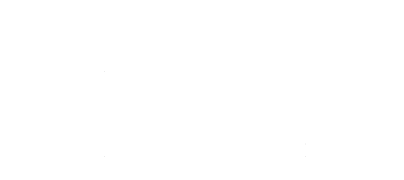
\includegraphics[width=0.75\linewidth]{1ion_Elevels.pdf}}
			\only<2>{\includegraphics[width=0.75\linewidth]{2ion_Elevels.pdf}}
			%\only<3>{\vspace{0.57em}}
			\[\hat{H}=-\frac{\hbar\omega_0}{2}\only<1>{\hat{\sigma}_z}\only<2>{\sum_i^n\hat{\sigma}_z^{(i)}} + \hbar\nu \left(\hat{a}^\dagger\hat{a} + \frac{1}{2}\right)\]
		\end{figure}
	\end{frame}
    \begin{frame}{Driving the system}
    	\begin{align*}
    		\onslide<1->{\hat{H}&=-\frac{\hbar\omega_0}{2}\sum_i^n\hat{\sigma}_z^{(i)}+ \hbar\nu \left(\hat{a}^\dagger\hat{a} + \frac{1}{2}\right) + \sum_{l}\frac{\Omega_l}{2}\hat{\sigma}_+^{\left(n_l\right)}e^{-i\left(\mathbf{kz}-\omega_l t\right)} + h.c.}\\
    		\onslide<2->{\hat{H}&=-\frac{\hbar\omega_0}{2}\sum_i^n\hat{\sigma}_z^{(i)}+ \hbar\nu \left(\hat{a}^\dagger\hat{a} + \frac{1}{2}\right) + \sum_{l}\frac{\Omega_l}{2}\hat{\sigma}_+^{\left(n_l\right)}e^{-i\left(\eta\left(\hat{a}+\hat{a}^\dagger\right) -\omega_l t\right)} + h.c.}\\
    		\onslide<3->{\hat{H}_I&=\sum_{l}\frac{\Omega_l}{2}\hat{\sigma}_+^{\left(n_l\right)}e^{-i\left(\eta\left(\hat{\tilde{a}}+\hat{\tilde{a}}^\dagger\right) -\Delta_l t\right)} + h.c.}
    	\end{align*}
    	\[\onslide<2->{\eta = \mathbf{kz_0}}\onslide<3->{\hspace{5em}\hat{\tilde{a}}=\hat{a}e^{-i\nu t}\hspace{5em}\hat{\tilde{a}}^\dagger =\hat{a}^\dagger e^{i\nu t}}\]
    \end{frame}

	\begin{frame}{Lamb-Dicke regime}
		\centering
		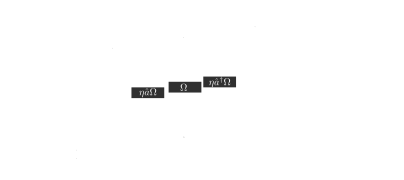
\includegraphics[width=0.75\linewidth]{Coupling_Elevels.pdf}
		{\[e^{i\eta\left(\hat{\tilde{a}}+\hat{\tilde{a}}^\dagger\right)}\approxeq\hat{\mathds{1}} + i\eta\left(\hat{\tilde{a}}+\hat{\tilde{a}}^\dagger\right) + \mathcal{O}\left(\eta^2\right)\]}
	\end{frame}

	\section{Driving schemes}
	\begin{frame}{M\o lmer-S\o rensen gate\footfullcite{MS-gate}}
		\centering
		\only<1>{\includegraphics[height=12em]{MS_gate_seq_OR.pdf}}
		\includegraphics[width=0.75\linewidth]{MS-gate.pdf}
	\end{frame}
	\begin{frame}{Strong coupling gate\footfullcite{SC2}}
		\centering
		\only<1>{\includegraphics[height=12em]{SC2_seq_OR.pdf}}
		\only<2>{\includegraphics[height=12em]{SC2_therm.pdf}}
		\only<3>{\includegraphics[height=12em]{SC2_seq.pdf}}
		\includegraphics[width=0.75\linewidth]{SC2-gate.pdf}
	\end{frame}
	\begin{frame}{Cardioid gate\footfullcite{Cardioid}}
		\centering
		\only<1>{\includegraphics[height=12em]{Cardioid_seq_OR.pdf}}
		\only<2>{\includegraphics[height=12em]{MS_Card_time_OR.pdf}}
		\only<3>{\includegraphics[height=12em]{Cardioid_seq.pdf}}
		\only<4>{\includegraphics[height=12em]{MS_Card_time.pdf}}
		\includegraphics[width=0.75\linewidth]{Cardioid-gate.pdf}
	\end{frame}
	\begin{frame}{Compound gate}
		\centering
		\only<1>{\includegraphics[height=12em]{Custom_SC2_seq_OR.pdf}}
		\only<2>{\includegraphics[height=12em]{Comp_time_OR.pdf}}
		\only<3>{\includegraphics[height=12em]{Comp_therm.pdf}}
		\only<4>{\includegraphics[height=12em]{Custom_SC2_seq.pdf}}
		\only<5>{\includegraphics[height=12em]{Comp_time.pdf}}
		\only<6>{\includegraphics[height=12em]{Comparison.pdf}}
		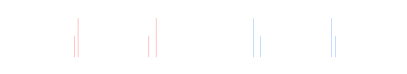
\includegraphics[width=0.75\linewidth]{Compound-gate.pdf}
		
		\vspace{0.70em}
	\end{frame}

	\section{Qubit frequency error}
	\begin{frame}{Dynamical decoupling}
		\begin{tabular*}{\linewidth}{c @{\extracolsep{\fill}} c}
			a & b \\
		\end{tabular*}
	\end{frame}

%	\begin{frame}{Comparison}
%		\centering
%		\includegraphics[height=12em]{Comparison.pdf}
%		\vspace{1.5em}
%	\end{frame}

%    \section*{Acknowledgments} %You can remove this if you do not want to use it
%        \begin{frame}{Acknowledgments}
%            The author is extremely thankful to Prof. Antônio F. R. T. Piza for the short, yet wonderful, conversations about this seminar.
%        \end{frame}

    \section{}
    \begin{frame}{}
        \centering
            \Huge\bfseries
        \textcolor{orange}{Thank you for the attention}
    \end{frame}

\end{document}
